\documentclass{article}
\usepackage[utf8x]{inputenc}
\usepackage{ucs}
\usepackage{amsmath} 
\usepackage{amsfonts}
\usepackage{upgreek}
\usepackage[english,russian]{babel}
\usepackage{graphicx}
\usepackage{float}
\usepackage{textcomp}
\usepackage{hyperref}
\usepackage{geometry}
  \geometry{left=2cm}
  \geometry{right=1.5cm}
  \geometry{top=1cm}
  \geometry{bottom=2cm}
\usepackage{tikz}
\usepackage{ccaption}
\usepackage{multicol}

\usepackage{listings}
%\setlength{\columnsep}{1.5cm}
%\setlength{\columnseprule}{0.2pt}


\begin{document}
\pagenumbering{gobble}

\lstset{
  language=C++,                % choose the language of the code
  basicstyle=\linespread{1.1}\ttfamily,
  columns=fixed,
  fontadjust=true,
  basewidth=0.5em,
  keywordstyle=\color{blue}\bfseries,
  commentstyle=\color{gray},
  stringstyle=\ttfamily\color{orange!50!black},
  showstringspaces=false,
  %numbers=false,                   % where to put the line-numbers
  numbersep=5pt,
  numberstyle=\tiny\color{black},
  numberfirstline=true,
  stepnumber=1,                   % the step between two line-numbers.        
  numbersep=10pt,                  % how far the line-numbers are from the code
  backgroundcolor=\color{white},  % choose the background color. You must add \usepackage{color}
  showstringspaces=false,         % underline spaces within strings
  captionpos=b,                   % sets the caption-position to bottom
  breaklines=true,                % sets automatic line breaking
  breakatwhitespace=true,         % sets if automatic breaks should only happen at whitespace
  xleftmargin=.2in,
  extendedchars=\true,
  keepspaces = true,
}
\lstset{literate=%
   *{0}{{{\color{red!20!violet}0}}}1
    {1}{{{\color{red!20!violet}1}}}1
    {2}{{{\color{red!20!violet}2}}}1
    {3}{{{\color{red!20!violet}3}}}1
    {4}{{{\color{red!20!violet}4}}}1
    {5}{{{\color{red!20!violet}5}}}1
    {6}{{{\color{red!20!violet}6}}}1
    {7}{{{\color{red!20!violet}7}}}1
    {8}{{{\color{red!20!violet}8}}}1
    {9}{{{\color{red!20!violet}9}}}1
}


\section*{Библиотека SFML. Graphical User Interface. Задачи.}

\begin{itemize}
\item \textbf{Перетаскивание:} В папке \texttt{1movable/} содержится заготовка исходного кода для этого задания. Эта программа просто рисует прямоугольник на экране. Сделайте его перетаскиваемым мышью. При нажатии на него и последующим движении мыши он должен начать двигаться вместе с курсором. При отпускании мыши должен остаться на месте.

\item \textbf{Карточки:} В этом же проекте создайте 20 прямоугольников случайного цвета, но одинакового размера, так чтобы все они были перетаскивыемыми.

\item \textbf{Выбор и удаление:} В папке \texttt{2move\_and\_delete/} содержится заготовка исходного кода для этого задания. В этой программе есть несколько объектов(кругов), которые можно выделять. Выделение происходит по нажатию левой клавиши мыши. Зажав клавишу \texttt{Ctrl} можно выделить несколько объектов. Также в программе реализован прямоугольник выделения (но он пока не выбирает объекты). Нажатием правой кнопки мыши можно создать случайный круг. Добавьте следующие возможности в программу:
	\begin{itemize}
	\item Перемещение всех выделенных объектов при зажатии левой клавиши мыши и её движении. Перемещаться должны все выделенные объекты параллельно (также как перемещаются несколько выделенных значков на рабочем столе). Прямоугольник выделения при этом рисоваться не должен.
	\item Выделение объектов с помощью прямоугольника выделения. Прямоугольник выделения должна рисоваться только если нажатие мыши произошло вне кругов. Все объекты, находящиеся внутри прямоугольника выделения, на момент отпускания левой кнопки мыши должны выделяться.
	\item При нажатии клавиши \texttt{Delete}, все выделенные объекты должны удаляться. Чтобы удалить элемент из \texttt{std::list} используйте итераторы и метод \texttt{erase}. \\
	Чтобы вспомнить как это работает -- пример работы с методом \texttt{erase} (удаляем все отрицательные числа):
	\begin{lstlisting}
	std::list<int> numbers = {5, -4, 6, 41, 64, -10, 16};
	for (std::list<int>::iterator it = numbers.begin(); it != numbers.end(); it++)
	{
		if (*it < 0)
			it = numbers.erase(it);
		// erase возвращает правильный итератор
		// Если удалять так numbers.erase(it) - цикл не сможет выполнить it++
	}
	\end{lstlisting}
	\item Задание случайного цвета. При нажатии клавиши пробел цвет всех выделенных шаров должен меняться на случайный. Для этого понадобится добавить поле \texttt{color} в класс \texttt{Ball}. 
	\end{itemize}

\item \textbf{Класс кнопки:} В папке \texttt{3button/} содержится заготовка исходного кода для этого задания.  Логика работы должна этой кнопки аналогичной логике работы обычной кнопки в ОС Windows. При нажатии на прямоугольник он немного меняет цвет. При отпускании мыши, если курсор всё ещё находится на прямоугольнике, срабатывает некоторое действие (печать в консоль).
	\begin{itemize}
	\item Создайте 1 круг. Сделайте так, чтобы при нажатии на кнопку цвет круга менялся бы на случайный.
	\item \textbf{Переключатель} - в этом же файле создайте класс под названием \texttt{ToggleButton}, который будет описывать поведение переключателя.
	\begin{center}
	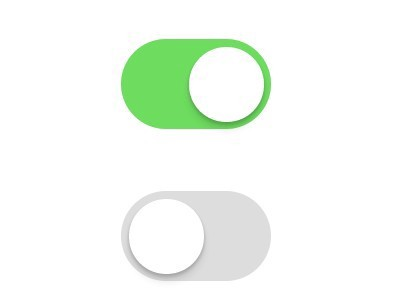
\includegraphics[scale=0.15]{../images/toggle_button.jpeg}
	\end{center}
	Переключатель может находится в 2-х состояниях (ON/OFF). При нажатии мышью на переключатель он должен менять состояние. Графическое оформление -- на ваше усмотрение.
	\item Создайте 1 экземпляр переключателя. Сделайте так, чтобы круг перекрашивался в зелёный цвет, если переключатель находится во включённом состоянии и так, чтобы круг перекрашивался в красный цвет, если переключатель выключен.
	\end{itemize}
	
\newpage
\item \textbf{Флажки:} В папке \texttt{4checkbox/} содержится заготовка исходного кода для этого задания. Описан класс \texttt{Checkbox} - флажка. Измените программу так, чтобы при нажатии на кнопку на экран печатались все города, у которых выделены флажки.

\item \textbf{Контекстное меню:} В папке \texttt{5context\_menu/} содержится пример, реализующий простейшее контекстное меню на SFML.
\begin{itemize}
\item Создайте круг. И добавьте опции в контекстное меню так, чтобы можно было менять цвет и размер круга.
\item Добавьте к задаче \textbf{Выбор и удаление} контекстное меню. С его помощью нужно создавать объекты, удалять их, изменять их цвет и радиус.

\end{itemize}


\end{itemize}

\end{document}